\section{Assessment 1 Segments}
U3 P2 Prepare a project specification\\
U3 P3 Prepare the procedures that will be followed when implementing the project\\
U3 P4 Use appropriate techniques to evaluate three potential solutions and select the best option for developement\\
U2 P7 Use appropriate ICT software package and hardware to present information\\
U3 P5 Outline the project solution and plans its implementation\\
.\\
U3 M2 Use a wide range of techniques and selection criteria to justify chosen solution\\
U2 M3 Evaluate the effectiveness of an ICT software package and its tools for preparation and presentation of information
.\\
U2 D2 Evaluate the use of an ICT presentation method and identify an alternative approach


\section{Initial Project Ideas}\textbf{2016/09/03}\\
I have been advised to for our initial ideas in a mind map\\
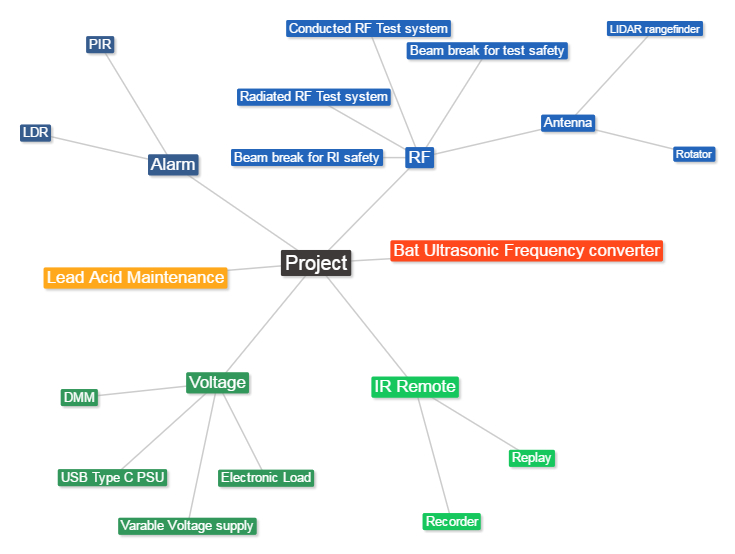
\includegraphics[width=\textwidth]{text_2_mind_map}

\section{Modus operandi}
Dates will be recorded in \gls{ISO8601} format\\
YYYY-MM-DDTHH:MM:ss+TZ:TZ\\
2016-11-25T16:20:50+00:00\\
The result of this every folder of name ordered files will be in date order\\
\\
Version control will be using the \gls{Git} version control system\\
\\
The specification MUST be defined by \gls{RFC2119}

\section{Engineering Project : Requirements}\textbf{2016/09/20}\\
The project consists or both project management and communications\\
This will require:\\
A logbook will all entries dated\\
Project specification\\
Logbook will itemise all communications:
\begin{itemize}
  \item Initial ideas and justification of project
  \item Specifications
  \item Technical drawings
  \item Schematic
  \item Calculations
  \item Component specification
  \item Simulation
  \item Planning
  \item Decisions
  \item Customer Communications
  \item Websites used
  \item Decision matrix for solutions
  \item SWOT analysis
  \item GANTT chart for planning / time-line
\end{itemize}


Have processes of
\begin{itemize}
  \item Specify
  \item Design
  \item Build
  \item Test
  \item Modify
  \item Evaluate
\end{itemize}

\section{Project : Selection Critical}\textbf{2016/09/27}\\
Should:\\
Provide something\\
Have design choices\\
Be achievable (could)\\
Possibly as I do in my workplace\\
Could use a project in work for project\\
 Where naturally accessible at work\\

\section{Project : Selection Criteria}\textbf{2016/10/04}\\
Could:\\
A physical product\\
A system product, a remote monitoring system\\
A service product, a engineering service\\
\\
Replication or extension of an existing product to enhance the service\\

\section{Project Selection}\textbf{2016/10/08}\\
I did some discovery work for a few of the project in my initial project ideas\\
IR Remote - nearly achieved before customer needs changed\\
Lidar has commercial modules available - down to timing accuracy\\
USB Type C PD specification is hundreds of pages long - too difficult\\

\section{Select solution}\textbf{2016/10/25}\\
Select from three solutions
This business sector has a couple of ready made platform products\\
LabVIEW by NI\\
VEE Pro by Keysight\\
Python 3 by Python Foundation\\
  With addition of some modules to communicate with test equipment\\

I am familiar with Python\\
I am using Python with instruments  already\\
This project should be viable for the use case\\
My employer already owns relevant hardware\\
I have access to expertise and relevant experience\\

\section{Project Final Idea}\textbf{2016/10/11}\\
RF Immunity test system\\
\begin{itemize}
  \item Control test equipment
  \item Monitor and control via feedback path
  \item Produce test report data
  \item Use Calibration factors
  \item Apply test standard \gls{EN61000-4-6:2014}
\end{itemize}
Customers will be test engineers at work\\


\section{Needs analysis}\textbf{2016/10/18}\\
To access is there a commercial or technical market\\
A survey may be used to derive a set of design specifications\\
Product performs in a repeatable manner\\
Product uses proven technology\\
Low incremental running cost : per runtime\\
Simple to maintain\\
Adaptable to new tests\\
Must stop/abort a test in a safe manner\\
Must apply correction factors\\

Project Specification from customer:\\
Time scale\\
Constraint dates\\
Availability of test set up for development\\
Plan installation\\
Set up drawing / work instructions\\


\section{Test process : Calculations for running test}\textbf{2016/11/01}\\
Calibrations are performed a higher amplitude than the test level\\
We need to calculate the level that we need to apply\\
Calibration\\

\begin{table}[h!]
\centering
\begin{tabular}{||c c c c||}
 \hline
 Frequency Hz & level V & siggen dBm & forward power dBm \\ [0.5ex]
 \hline
 150e3 & 18 & -9 & 38.64 \\
 200e3 & 18 & -9 & 38.46 \\
 \hline
\end{tabular}
\caption{Example Calibration data}
\label{table:1}
\end{table}

.\\
For a calibration performed at 18V\\
For a test run to be performed at 10V\\
Offset V = Calibration power V : Wanted power V\\
Offset dBm = V2dBm(offset dBm)\\
Target forward power = forward power dBm : Offset dBm\\

Levelling performed without and with any AM applied\\
Dwell for time in both CW and AM modulation?\\

\section{Estimated time}\textbf{2016/11/08}\\\lstinputlisting[language=Python, caption=Estimated Time]{py_estimatedtime.py}

\section{Unit conversion}\textbf{2016/11/08}\\
Power meters operate in units of Watts or dBm\\
Our target level for calibration is in Volts\\
Our meter has best linearity in Watts\\
Therefore conversion between Watts and Volts is required\\
\lstinputlisting[language=Python, caption=Power meter calculations]{py_powermetercalcs.py}

\section{Project Specification Revised}\textbf{2016/11/15}\\

Functional requirements when running a test\\
Instrument control\\
  Power meter\\
  Signal generator\\
Step frequency steps\\
Use/apply calibration factors\\
Calculate the expected power with given CDN factors at coupling point\\
Level with given tolerance to calculated power\\
Dwell time must be at-least minimum time\\
Display a plot during test\\
Have a mode of operation for validating an EUT fault\\
  mini sweep over last n points\\
Pause standby a test\\
Stop a test\\


\section{Project discussion with Stuart}\textbf{2016/11/22}\\
Discussed project with Stuart\\
Identified additional documentation requirements\:\\
Terminology\\
Test configurations\\
The installation and operation of the software MUST be repeatable for a given build\\
\begin{table}[h!]
\centering
\begin{tabular}{||c c c c c c c c||}
 \hline
 Criteria & Weighting & LabVIEW & VEEPro & Python & LabVIEW & VEEPro & Python \\ [0.5ex]
 \hline
 Costs & 5 & 2 & 4 & 8 & 10 &	20 & 40 \\
 Implementation ease & 3 & 4 & 1 & 7 & 12 & 3 & 21 \\
Machine tools available & 7 & 6 & 1 & 10  & 42 & 7 & 70 \\
Project deadline risk & 7 & 3 & 1 & 6 & 21 & 7 & 42 \\
Material availability & 5 & 6 & 2 & 10 & 30 & 10 & 50 \\
H \& S \& Risk assessment & 4 & 5 & 5 & 5 & 20 & 20 & 20 \\
Expertise to complete & 5 & 3 & 1 & 7 & 15 & 5 & 35 \\
Totals & 36 & . & . & . & 150 & 72 & 278 \\
\hline
\end{tabular}
\caption{Decision making table}
\label{table:4}
\end{table}
\textbf{2016/11/20}\\
\section{SWOT Analysis}\textbf{2016/11/27}\\
\begin{tikzpicture}[
    any/.style={minimum width=8cm,minimum height=8cm,%
                 text width=7.5cm,align=center,outer sep=0pt},
    header/.style={any,minimum height=1cm,fill=black!10},
    leftcol/.style={header,rotate=90},
    mycolor/.style={fill=#1, text=#1!60!black}
]

\matrix (SWOT) [matrix of nodes,nodes={any,anchor=center},%
                column sep=-\pgflinewidth,%
                row sep=-\pgflinewidth,%
                row 1/.style={nodes=header},%
                column 1/.style={nodes=leftcol},
                inner sep=0pt]
{
          &|[fill=helpful]| {\texta} & |[fill=harmful]| {\textb} \\
|[fill=internal]| {\textcn} & |[mycolor=S]| & |[mycolor=W]| \\
|[fill=external]| {\textdn} & |[mycolor=O]| & |[mycolor=T]| \\
};

\node[any, anchor=center] at (SWOT-2-2) {Project will build on existing experience\\Can reuse some existing code\\};
\node[any, anchor=center] at (SWOT-2-3) {Experence with control faults\\Experience with larger scale applications\\};
\node[any, anchor=center] at (SWOT-3-2) {Low operational expense\\ No Licensing expense from this project\\ };
\node[any, anchor=center] at (SWOT-3-3) {Intgeration with existing testing platform\\};

\end{tikzpicture}


\newpage
\section{Setup Diagrams}\textbf{2016/11/22}\\
Diagram showing Normal testing set-up and calibration set-up\\
\begin{table}[h!]
\centering
\begin{tabular}{||c c c c c||}
\hline
& & & & Supply \\
& & & & Pwr/Signal line \\
Signal Generator & RF Amplifier & Coupler & Atten & CDN \\
& & Cable/Atten & & Pwr/Signal line \\
& & Power Head & & EUT \\
& & Power Meter & & \\
\hline
\end{tabular}
\caption{Test configuration}
\label{table:3}
\end{table}

\begin{table}[h!]
\centering
\begin{tabular}{||c c c c c||}
\hline
& & & & 150 Ohms termination \\
Signal Generator & RF Amplifier & Coupler & Atten & CDN \\
& & Cable/Atten & & 100Ohms through \\
& & Power Head  & & 10dB Power Atten \\
& & Power Meter & & 10dB Atten \\
& & & & Calibration Power Head \\
& & & & Calibration Power Meter \\
\hline
\end{tabular}
\caption{Calibration configuration}
\label{table:4}
\end{table}


\section{Get data from a power meter}\textbf{2016/12/6}\\
\lstinputlisting[language=Python, caption=Power meter data]{py_getpowermeterdata.py}

\section{Step frequency steps}\textbf{2016/12/13}\\
\lstinputlisting[language=Python, caption=Frequency Steps]{py_frequencysteps.py}

Consider adding interesting frequency points
Need to be able to rewind by a number of steps

\section{TODO}
\subsection{Validation of new software, Primary function}
The software needs to be evaluated in comparison with the existing software with respect with the primary test function\\
An validation comparison method needs to be designed and tested\\

Calculate if the 0.1 - 1000MHz Amplifier Research amplifier has sufficient power for 3V target\\
Initial comparisons can be performed with a similar coupler into a termination load\\
The variation of the impedance may result in a different response with the existing software\\
But both software installations must respond the same way within limits\\


\subsection{Parse existing cal data}
\subsection{Get / set data from a signal generator}
\subsection{Limit ramping up signal generator}
\subsection{Abort test}
\subsection{Pause off test}
\subsection{Rewind test - validate EUT fault}
\subsection{Display table during test - of last ten points}
\subsection{Display graph during test}
\subsection{Monitor line voltage during test}
\subsection{Exception handling}
Should store state and back trace when encountered unless deliberately handled\\

\newpage\section{About}\section{About Python}
\label{sec:Python}
\gls{Python} is a programming language available from \href{https://python.org}{Python.org}\\

Windows XP support ended with 3.4.4\\
Otherwise always use the highest numbered version\\

When installing Python offers to include the runtime in PATH always set this option on\\
Otherwise you need to invoke the Python runtime with the full path every time\\

Extra Python functionality is built up of modules available from \gls{Pypi} or \gls{Git}\\
These modules are installable via \gls{pip}\\

For example:\\
\`pip install pyserial\`\\
Installs the module to utilise serial ports and includes a small serial terminal application.\\

\gls{venv} is a module that is part of the Python core that creates Python virtual environments\\
This venv can be used to install modules separately from the system installation\\
If used correctly this allows programs to be reliably installed and this provides reasonable assurance that the program will operate the same way on a different computer\\

Python is a programming language that uses tabs to delineate nested flow control\\

I have written a number of .bat scripts to install, start, run, (Utilities, Serial console, GPIB console, Code checkers)\\
\subsection{RFC2119}
\label{sec:RFC2119}
\gls{RFC2119} is a available from \href{https://tools.ietf.org/html/rfc2119}{IETF.org}\\

The remainder of this section is a extract of \href{https://tools.ietf.org/html/rfc2119}{IETF.org RFC 2119}
By: S. Bradner, Harvard University, March 1997\\

Abstract\\

   In many standards track documents several words are used to signify
   the requirements in the specification.  These words are often
   capitalized.  This document defines these words as they should be
   interpreted in IETF documents.  Authors who follow these guidelines
   should incorporate this phrase near the beginning of their document:\\

      The key words "MUST", "MUST NOT", "REQUIRED", "SHALL", "SHALL
      NOT", "SHOULD", "SHOULD NOT", "RECOMMENDED",  "MAY", and
      "OPTIONAL" in this document are to be interpreted as described in
      RFC 2119.\\

   Note that the force of these words is modified by the requirement
   level of the document in which they are used.\\

1. MUST   This word, or the terms "REQUIRED" or "SHALL", mean that the
   definition is an absolute requirement of the specification.\\

2. MUST NOT   This phrase, or the phrase "SHALL NOT", mean that the
   definition is an absolute prohibition of the specification.\\

3. SHOULD   This word, or the adjective "RECOMMENDED", mean that there
   may exist valid reasons in particular circumstances to ignore a
   particular item, but the full implications must be understood and
   carefully weighed before choosing a different course.\\

4. SHOULD NOT   This phrase, or the phrase "NOT RECOMMENDED" mean that
   there may exist valid reasons in particular circumstances when the
   particular behavior is acceptable or even useful, but the full
   implications should be understood and the case carefully weighed
   before implementing any behavior described with this label.\\

5. MAY   This word, or the adjective "OPTIONAL", mean that an item is
  truly optional.  One vendor may choose to include the item because a
  particular marketplace requires it or because the vendor feels that
  it enhances the product while another vendor may omit the same item.
  An implementation which does not include a particular option MUST be
  prepared to interoperate with another implementation which does
  include the option, though perhaps with reduced functionality. In the
  same vein an implementation which does include a particular option
  MUST be prepared to interoperate with another implementation which
  does not include the option (except, of course, for the feature the
  option provides.)\\

6. Guidance in the use of these Imperatives\\

  Imperatives of the type defined in this memo must be used with care
  and sparingly.  In particular, they MUST only be used where it is
  actually required for interoperation or to limit behavior which has
  potential for causing harm (e.g., limiting retransmisssions)  For
  example, they must not be used to try to impose a particular method
  on implementors where the method is not required for
  interoperability.\\
\subsection{Git}
\label{sec:Git}
Git is a fast version control system\\
Nearly all operations occur locally\\
Distributed, clones (replicas) are by default full copys of the project history\\
Users commit into a repository, repository’s have checksums for each file in a commit and respective metadata\\
Ergo modifying history will invalidate checksums in a provable way\\

Diffs for text based files or files that can be presented in a textual manner, can have diffs that represent the changes from the current master to the files in the working area\\

